

\begin{frame}{\ft{A3R Applications as Research Objects}}

\doubleFrame{Complementary to the benefits of native applications 
for \q{obtaining} data, A3R components are also 
powerful tools for showing and analyzing research findings.}

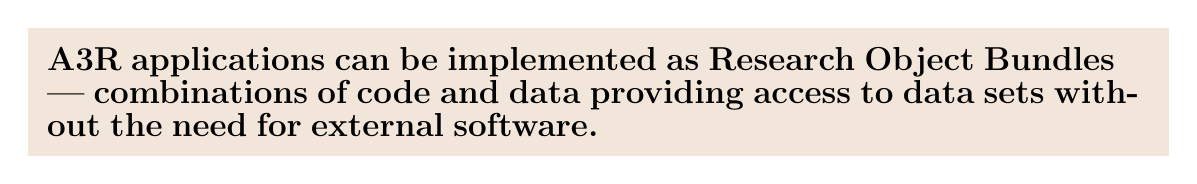
\begin{tikzpicture}
\nodeincludegraphicsTR{2.7cm}{2cm}{pics/Res-4.png}

 \node [anchor=west,fill=brown!20!white,inner sep=7, text width=14cm]
  (longnote) at (5.5,7) {%  %{\color{rb!85!red}{
  {\cframedbox{\large \textbf{A3R applications can be implemented 
as \q{Research Object Bundles} --- combinations of code and data 
providing access to data sets without the need for external software.}}}};

\end{tikzpicture}


\end{frame}

